\documentclass[10pt]{beamer}

% Beamer style
%\usetheme[secheader]{Madrid}
% \usetheme{CambridgeUS}
\useoutertheme{infolines}
\usecolortheme[rgb={0.65,0.15,0.25}]{structure}
% \usefonttheme[onlymath]{serif}
\beamertemplatenavigationsymbolsempty
%\AtBeginSubsection

% Packages
%\usepackage[french]{babel}
\usepackage[latin1]{inputenc}
\usepackage{color}
\usepackage{xspace}
%\usepackage{dsfont, stmaryrd}
\usepackage{amsmath, amsfonts, amssymb}
\usepackage{epsfig}
\usepackage{url}
\usepackage{/home/robin/LATEX/Biblio/astats}
%\usepackage[all]{xy}
\usepackage{graphicx}

% Commands
\definecolor{darkred}{rgb}{0.65,0.15,0.25}
%\newcommand{\emphase}[1]{\textcolor{darkred}{#1}}
\newcommand{\emphase}[1]{{#1}}
\newcommand{\paragraph}[1]{\textcolor{darkred}{#1}}
\newcommand{\refer}[1]{{\footnotesize{\textcolor{gray}{{\cite{#1}}}}}}
\newcommand{\Refer}[1]{{\footnotesize{\textcolor{gray}{{#1}}}}}
\renewcommand{\newblock}{}

% Symbols
\newcommand{\Abf}{{\bf A}}
\newcommand{\Beta}{\text{B}}
\newcommand{\Bcal}{\mathcal{B}}
\newcommand{\BIC}{\text{BIC}}
\newcommand{\Ccal}{\mathcal{C}}
\newcommand{\dd}{\text{~d}}
\newcommand{\dbf}{{\bf d}}
\newcommand{\Dcal}{\mathcal{D}}
\newcommand{\Esp}{\mathbb{E}}
\newcommand{\Ebf}{{\bf E}}
\newcommand{\Ecal}{\mathcal{E}}
\newcommand{\Gcal}{\mathcal{G}}
\newcommand{\Gam}{\mathcal{G}\text{am}}
\newcommand{\Hcal}{\mathcal{H}}
\newcommand{\Ibb}{\mathbb{I}}
\newcommand{\Ibf}{{\bf I}}
\newcommand{\ICL}{\text{ICL}}
\newcommand{\Cov}{\mathbb{C}\text{ov}}
\newcommand{\Corr}{\mathbb{C}\text{orr}}
\newcommand{\Var}{\mathbb{V}}
\newcommand{\Vsf}{\mathsf{V}}
\newcommand{\pen}{\text{pen}}
\newcommand{\Fcal}{\mathcal{F}}
\newcommand{\Hbf}{{\bf H}}
\newcommand{\Jcal}{\mathcal{J}}
\newcommand{\Kbf}{{\bf K}}
\newcommand{\Lcal}{\mathcal{L}}
\newcommand{\Mcal}{\mathcal{M}}
\newcommand{\mbf}{{\bf m}}
\newcommand{\mum}{\mu(\mbf)}
\newcommand{\Ncal}{\mathcal{N}}
\newcommand{\Nbf}{{\bf N}}
\newcommand{\Nm}{N(\mbf)}
\newcommand{\Ocal}{\mathcal{O}}
\newcommand{\Obf}{{\bf 0}}
\newcommand{\Omegas}{\underset{s}{\Omega}}
\newcommand{\Pbf}{{\bf P}}
\newcommand{\Pt}{\widetilde{P}}
\newcommand{\Pcal}{\mathcal{P}}
\newcommand{\Qcal}{\mathcal{Q}}
\newcommand{\Rbb}{\mathbb{R}}
\newcommand{\Rcal}{\mathcal{R}}
\newcommand{\Scal}{\mathcal{S}}
\newcommand{\Ucal}{\mathcal{U}}
\newcommand{\Vcal}{\mathcal{V}}
\newcommand{\BP}{\text{BP}}
\newcommand{\EM}{\text{EM}}
\newcommand{\VEM}{\text{VEM}}
\newcommand{\VBEM}{\text{VBEM}}
\newcommand{\cst}{\text{cst}}
\newcommand{\obs}{\text{obs}}
\newcommand{\ra}{\emphase{\mathversion{bold}{$\rightarrow$}~}}
%\newcommand{\transp}{\text{{\tiny $\top$}}}
\newcommand{\transp}{\text{{\tiny \mathversion{bold}{$\top$}}}}
\newcommand{\logit}{\text{logit}\xspace}

% Directory
\newcommand{\figmixt}{/home/robin/ENSEIGN/COURS/MELANGE}
\newcommand{\figbma}{/home/robin/RECHERCHE/RUPTURES/MELANGE/Exemples/Grippe}
\newcommand{\fignet}{../FIGURES}
\newcommand{\figeco}{/home/robin/RECHERCHE/ECOLOGIE/EXPOSES/FIGURES}
%\newcommand{\figmotif}{/home/robin/RECHERCHE/RESEAUX/Motifs/FIGURES}


%====================================================================
%====================================================================

%====================================================================
%====================================================================
\begin{document}
%====================================================================
%====================================================================

%====================================================================
\frame{\frametitle{Properties of variational estimates for SBM}

  \paragraph{Credibility intervals:}   $\pi_1$: $+$,
  $\gamma_{11}$: \textcolor{red}{$\triangle$}, $\gamma_{12}$:
  \textcolor{blue}{$\circ$}, $\gamma_{22}$: \textcolor{green}{$\bullet$} \\
%   $$
  \includegraphics[width=1\textwidth]{../FIGURES/im-ICQ2-2-new} \\
}

%====================================================================
\frame{\frametitle{VBEM inference for SBM: {\sl E. coli}'s operon network}

  \vspace{-0.5cm}
  \hspace{-0.5cm}
  \begin{tabular}{cc}         
    \begin{tabular}{p{0.45\textwidth}}
       \vspace{-1cm}
       \includegraphics[width=.45\textwidth]{\fignet/im_EcoliVEM_2} \\
       %~\\
       \refer{PMD09}
    \end{tabular}
    &
    \begin{tabular}{p{0.45\textwidth}}
      \vspace{-.3cm}
      \paragraph{Meta-graph representation.} \\
      %\vspace{-.02\textwidth}
      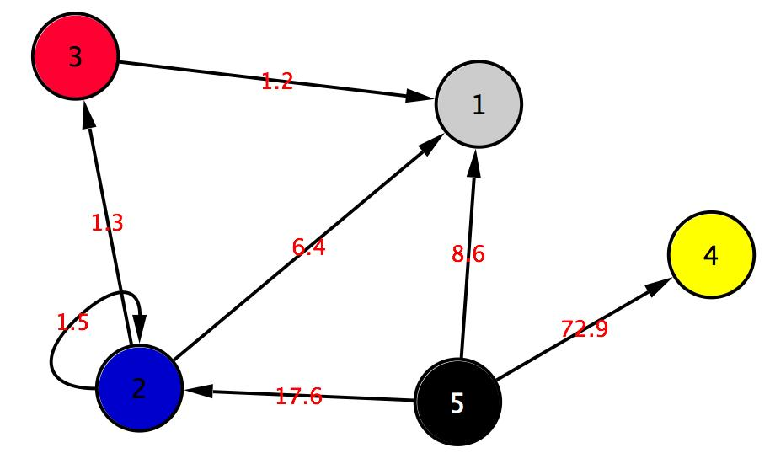
\includegraphics[width=.35\textwidth]{\fignet/VEMmetagraphe}  \\
      \vspace{-.3cm}
      \paragraph{Parameter estimates.} $K = 5$     \\
      \includegraphics[width=.35\textwidth]{../FIGURES/im-pi1BVEM}\\        
      \includegraphics[width=.35\textwidth]{../FIGURES/im-pi2BVEM}\\
      \includegraphics[width=.35\textwidth]{../FIGURES/im-pi3BVEM}\\
      \includegraphics[width=.35\textwidth]{../FIGURES/im-pi4BVEM}\\
      \includegraphics[width=.35\textwidth]{../FIGURES/im-pi5BVEM}\\
      \hline 
      \includegraphics[width=.35\textwidth]{../FIGURES/im-alphaBVEM}\\
    \end{tabular}
  \end{tabular}
  }

%====================================================================
\frame{\frametitle{Interpreting the graphon function}

  \bigskip \bigskip 
  \centerline{
  \begin{tabular}{ccc}
  'Scale free' & Community & Small world \\
  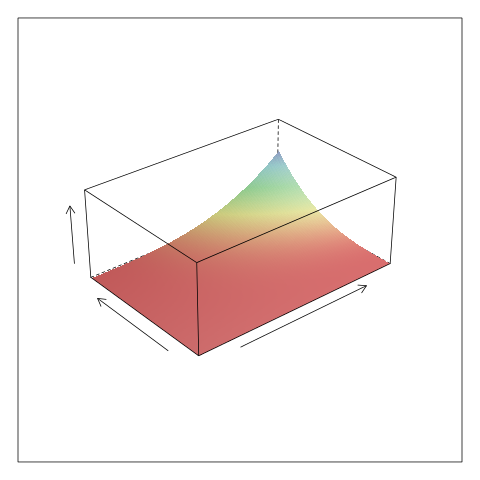
\includegraphics[width=.3\textwidth]{../FIGURES/EDD-ScaleFreeTrueGraphon} &
  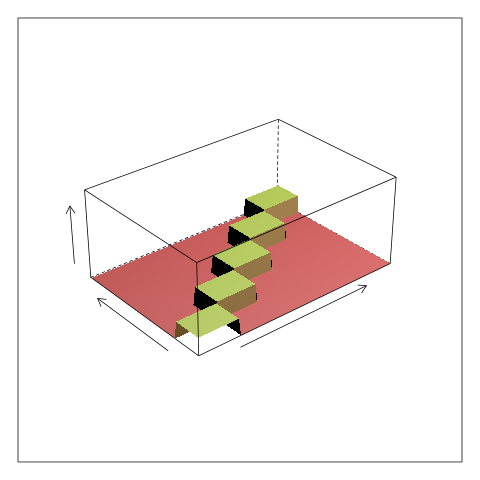
\includegraphics[width=.3\textwidth]{../FIGURES/CommunityTrueGraphon} &
  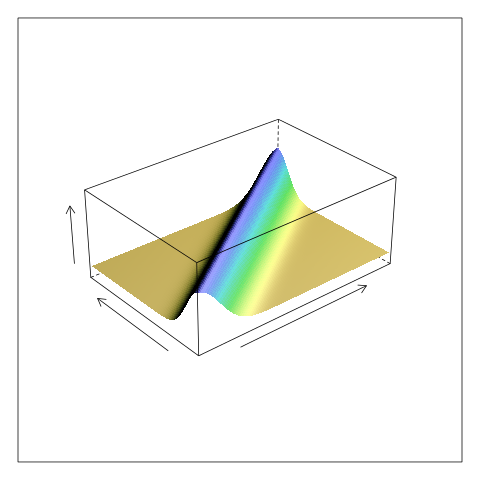
\includegraphics[width=.3\textwidth]{../FIGURES/SmallWorldTrueGraphon} 
  \end{tabular}
  } 
  
  \bigskip 
  \paragraph{Remark:} $\gamma(\cdot, \cdot) = $cst \ra ER model

}

%====================================================================
\subsection*{Variational Bayes inference for $W$-graph}
%====================================================================
\frame{ \frametitle{SBM as a $W$-graph model}

$$
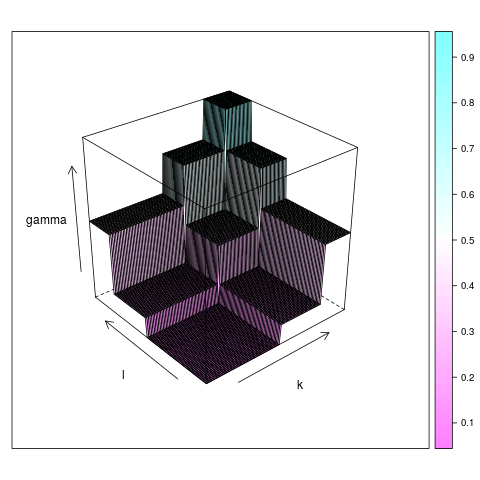
\includegraphics[width=.5\textwidth]{../FIGURES/FigCLADAG-SBM-graphon}
$$
}

%====================================================================
\frame{ \frametitle{Variational Bayes estimation of $\gamma(z, z')$}

Posterior mean $\widetilde{\Esp}(\gamma^{SBM}_K(z, z') | Y, K)$ 
$$
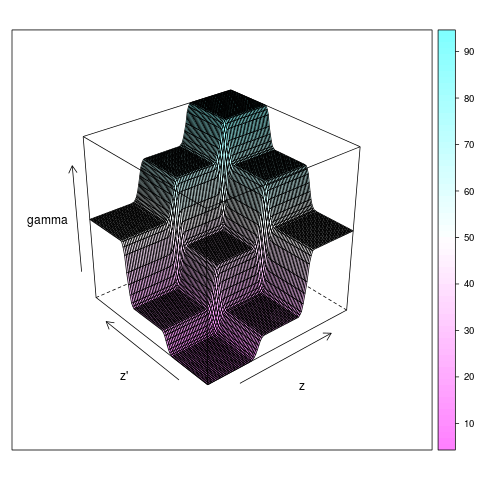
\includegraphics[width=.5\textwidth]{../FIGURES/FigGraphon-SBM-average}
$$
}

%====================================================================
\frame{\frametitle{Ecological network between fungal species}

  Link between 2 fungi if they are observed on one common host.

  \begin{tabular}{cc}
    \begin{tabular}{p{.5\textwidth}}
	 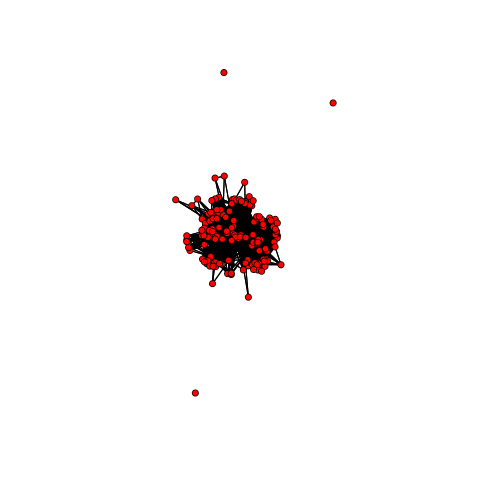
\includegraphics[width=.45\textwidth]{../FIGURES/Fungi-graph}
    \end{tabular}
    & 
    \hspace{-.1\textwidth}
    \begin{tabular}{p{.5\textwidth}}
	 \begin{overprint}
	 \onslide<1>
	 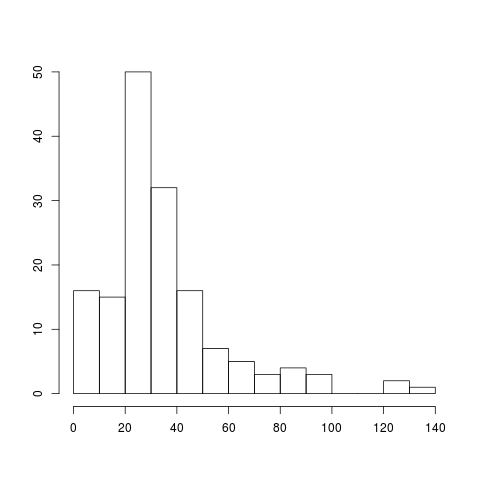
\includegraphics[width=.45\textwidth]{../FIGURES/Fungi-degree}
	 \onslide<2>
	 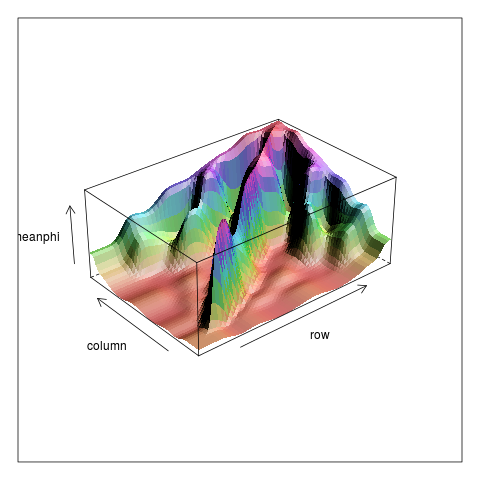
\includegraphics[width=.45\textwidth]{../FIGURES/Fungi-graphon}
	 \end{overprint}
    \end{tabular}
  \end{tabular}
}

%====================================================================
\frame{\frametitle{Brain network}

  Links = connexions between areas of the macaque's cortex

  \begin{tabular}{cc}
    \begin{tabular}{p{.5\textwidth}}
	 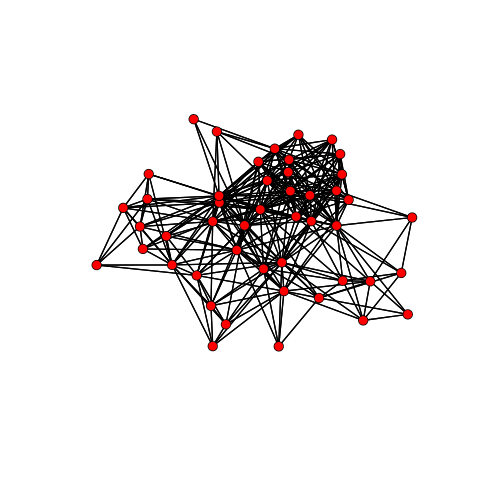
\includegraphics[width=.45\textwidth]{../FIGURES/Macaque-graph}
    \end{tabular}
    & 
    \hspace{-.1\textwidth}
    \begin{tabular}{p{.5\textwidth}}
	 \begin{overprint}
	 \onslide<1>
	 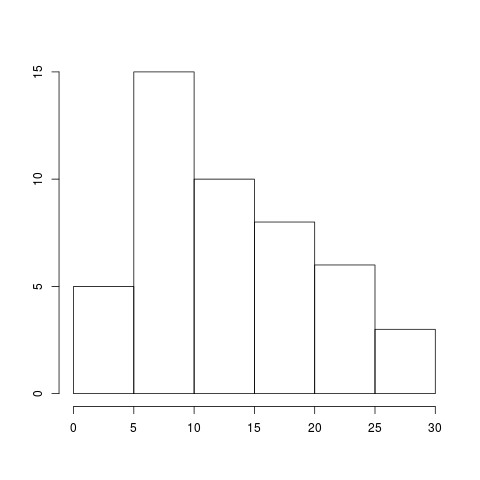
\includegraphics[width=.45\textwidth]{../FIGURES/Macaque-degree}
	 \onslide<2>
	 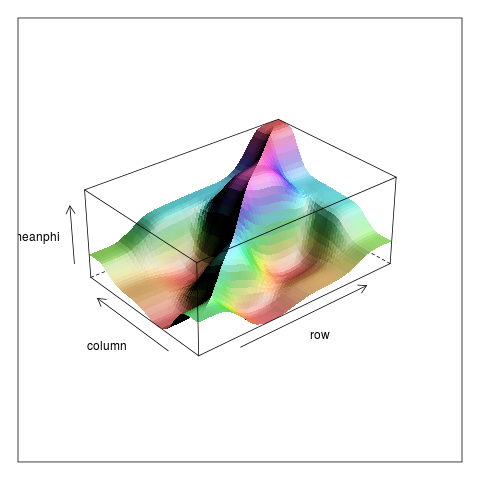
\includegraphics[width=.45\textwidth]{../FIGURES/Macaque-graphon}
	 \end{overprint}
    \end{tabular}
  \end{tabular}
}

%====================================================================
\frame{\frametitle{Blog network}

  Links = connexions between French political blogs

  \begin{tabular}{cc}
    \begin{tabular}{p{.5\textwidth}}
	 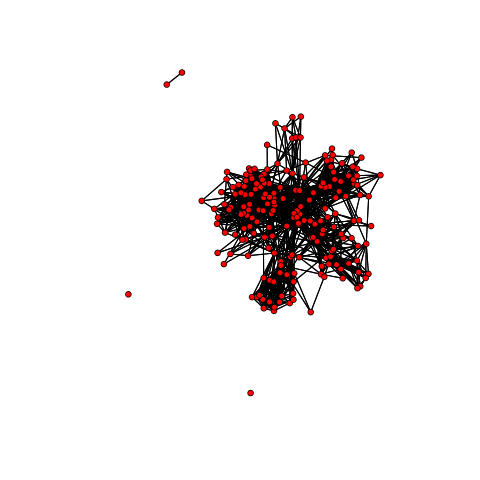
\includegraphics[width=.45\textwidth]{../FIGURES/Blog-graph}
    \end{tabular}
    & 
    \hspace{-.1\textwidth}
    \begin{tabular}{p{.5\textwidth}}
	 \begin{overprint}
	 \onslide<1>
	 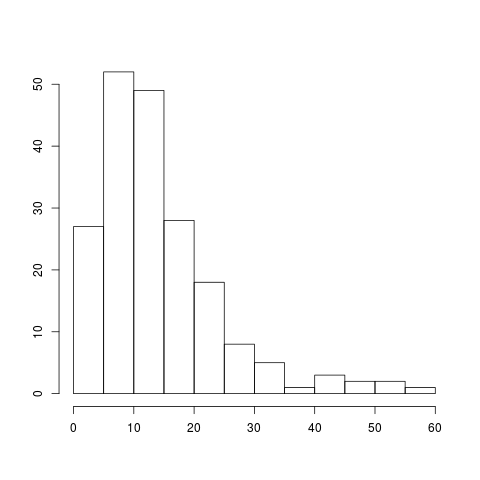
\includegraphics[width=.45\textwidth]{../FIGURES/Blog-degree}
	 \onslide<2>
	 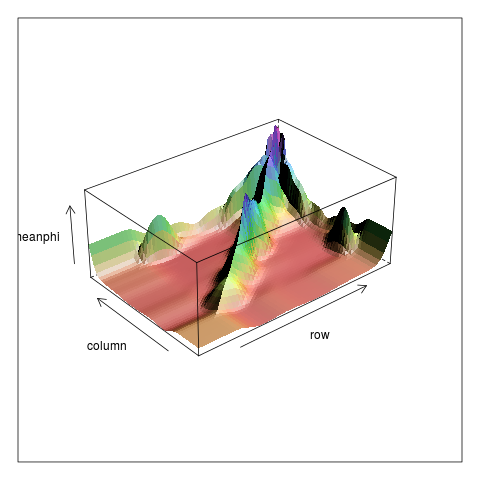
\includegraphics[width=.45\textwidth]{../FIGURES/Blog-graphon}
	 \end{overprint}
    \end{tabular}
  \end{tabular}
}

%====================================================================
\frame{ \frametitle{Network frequencies in the blog network}

% \vspace{-0.1\textheight}
$$
\begin{tabular}{crrrr}
  \hline
 Motif & Count & Mean & Std. dev. \\ % & approx $p$-value \\ 
 & ($\times 10^3$) & ($\times 10^3$) & ($\times 10^3$) \\ % & \refer{PDK08} \\ 
  \hline
  \begin{tabular}{c} 
\includegraphics[width=.045\textwidth]{../FIGURES/FigMotif-I} \end{tabular} & 29.7 & 39.7 & 8.3 \\ % & 0.89 \\ 
  \begin{tabular}{c} 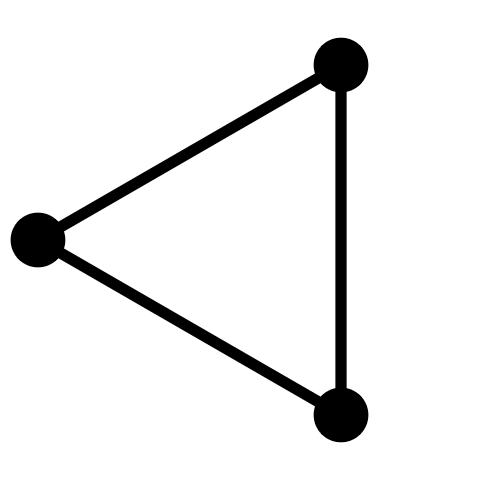
\includegraphics[width=.045\textwidth]{../FIGURES/FigMotif-Triangle} \end{tabular} & 3.8 & 4.6 & 1.3 \\ % & 0.69 \\ 
  \begin{tabular}{c} 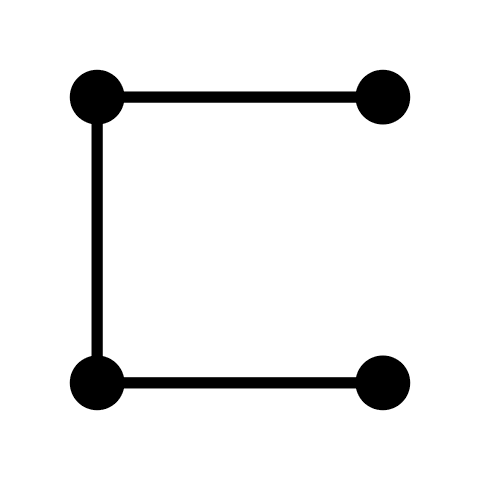
\includegraphics[width=.045\textwidth]{../FIGURES/FigMotif-Chain4} \end{tabular} & 608.7 & 968.3 & 336.8 \\ % & 0.86 \\ 
  \begin{tabular}{c} 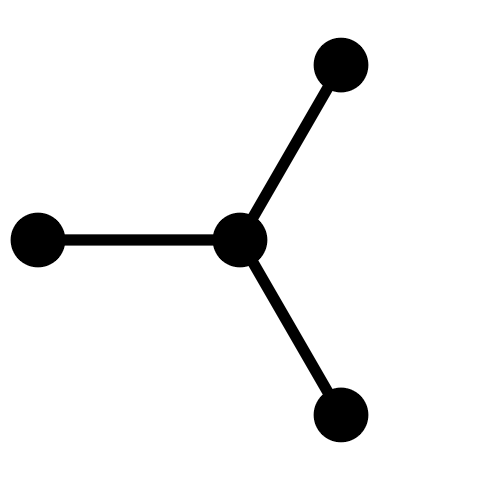
\includegraphics[width=.045\textwidth]{../FIGURES/FigMotif-Star3} \end{tabular}  & 279.8 & 428.9 & 154.0 \\ % & 0.83 \\ 
  \begin{tabular}{c} 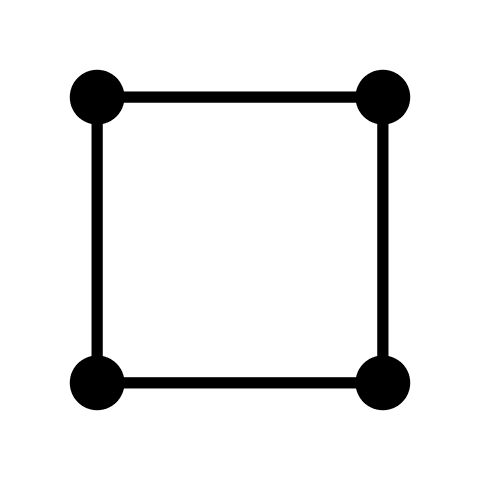
\includegraphics[width=.045\textwidth]{../FIGURES/FigMotif-Square} \end{tabular} & 47.4 & 74.5 & 35.1 \\ % & 0.77 \\ 
  \begin{tabular}{c} 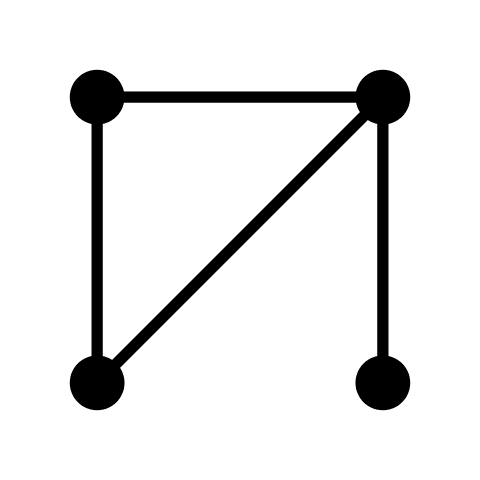
\includegraphics[width=.045\textwidth]{../FIGURES/FigMotif-Whisker} \end{tabular} & 270.5 & 397.0 & 177.0 \\ % & 0.75 \\ 
  \begin{tabular}{c} 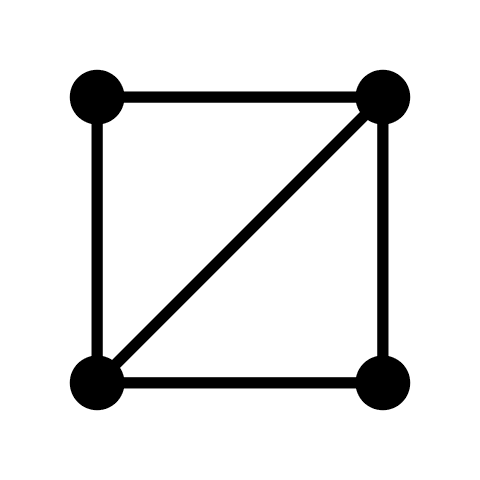
\includegraphics[width=.045\textwidth]{../FIGURES/FigMotif-SquareDiag} \end{tabular} & 62.1 & 87.8 & 47.4 \\ % & 0.67 \\ 
  \begin{tabular}{c} 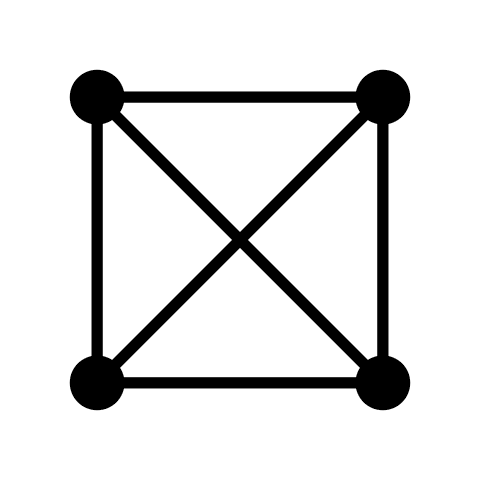
\includegraphics[width=.045\textwidth]{../FIGURES/FigMotif-Clique4} \end{tabular} & 6.5 & 8.8 & 5.4 \\ % & 0.61 \\ 
   \hline
\end{tabular}
$$

No specific structure seems to be exceptional wrt the model's expectations.

}

%====================================================================
\frame{ \frametitle{Tree network}

  \newcommand{\GOFplot}{/home/robin/Dropbox/vbemapp/gof2/jcgs/figures}
  
  \paragraph{Regression:} covariates = genetic distance, taxonomic distance, geographic distance
 
  \bigskip
  \begin{tabular}{cc} 
   $\arg\max_K \Pt(K|Y) = 9$ & \hspace{-.1\textwidth} $\arg\max_K \Pt(K|Y) = 3$\\
   ~\\
    \begin{tabular}{p{.5\textwidth}}
     \includegraphics[width=.4\textwidth]{\GOFplot/treed0}    
     \end{tabular}
    & \hspace{-.1\textwidth}
    \begin{tabular}{p{.5\textwidth}}
     \includegraphics[width=.4\textwidth]{\GOFplot/treed3}
    \end{tabular}
  \end{tabular}
}

%====================================================================
\frame{ \frametitle{Blog network}

  \newcommand{\GOFplot}{/home/robin/Dropbox/vbemapp/gof2/jcgs/figures}

  \paragraph{Regression:} covariates = same political party, pair includes a journalist
  
  \bigskip
  \begin{tabular}{cc} 
   $\arg\max_K \Pt(K|Y) = 12$ & \hspace{-.1\textwidth} $\arg\max_K \Pt(K|Y) = 5$\\
   ~\\
    \begin{tabular}{p{.5\textwidth}}
     \includegraphics[width=.4\textwidth]{\GOFplot/blogd0}    
     \end{tabular}
    & \hspace{-.1\textwidth}
    \begin{tabular}{p{.5\textwidth}}
     \includegraphics[width=.4\textwidth]{\GOFplot/blogd3}
    \end{tabular}
  \end{tabular}

}

%====================================================================
\frame{ \frametitle{Florentine families business network}

  \newcommand{\GOFplot}{/home/robin/Dropbox/vbemapp/gof2/jcgs/figures}

  \paragraph{Regression:} covariates = wealth, number of seats in councils, number of marriage ties
  
  \bigskip
  \begin{tabular}{cc} 
%    $\arg\max_K \Pt(K|Y) = 12$ & \hspace{-.1\textwidth} $\arg\max_K \Pt(K|Y) = 5$\\
%    ~\\
    \begin{tabular}{p{.5\textwidth}}
     \includegraphics[width=.4\textwidth]{\GOFplot/businessd0}    
     \end{tabular}
    & \hspace{-.1\textwidth}
    \begin{tabular}{p{.5\textwidth}}
     \includegraphics[width=.4\textwidth]{\GOFplot/businessd3}
    \end{tabular}
  \end{tabular}

}

%====================================================================
%====================================================================
\end{document}
%====================================================================
%====================================================================

  \begin{tabular}{cc}
    \begin{tabular}{p{.5\textwidth}}
    \end{tabular}
    & 
    \hspace{-.02\textwidth}
    \begin{tabular}{p{.5\textwidth}}
    \end{tabular}
  \end{tabular}

